\chapter*{前言}
\addcontentsline{toc}{chapter}{前言}

近代数学的一个特点是公理化、结构化。
代表近代数学的布尔巴基(Bourbaki)学派认为“数学是研究抽象结构的学科”,
这与恩格斯的观点“数学是关于现实世界数量关系和空间形式的科学”略有出入。
本讲义力图介绍近代数学中的四大基本结构:序结构、代数结构、拓扑结构、测度结构,
从而勾勒出近代数学基本框架,满足那些“想要多学一些数学”的爱好者们的基本需求,
并为其进一步学习近代数学奠定基础。

虽说声称是“零基础入门高等数学”,
本讲义其实并不是真正的“白手起家”,
还是要假定读者对一些基本的数学对象有直观的了解,
包括:实数的加减乘除运算、实数大小的比较,仅此而已。

事实上,近代数学基础完整的构建顺序大概是:命题逻辑$\rightarrow$
一阶谓词逻辑$\rightarrow$公理集合论$\rightarrow$自然数公理系统
$\rightarrow$实数理论。什么是自然数中的“0”,什么是“1”,
“自然数”是在集合论的框架下定义出来的,并不是“本来就有的”;
而自然数的加法运算也是定义出来的,
不再是初等数学那样子来源于日常生活经验,理所当然的。
这也是为什么罗素用了300多页才得到了自然数“1”的定义,这才是真正的“白手起家”。
有了自然数,之后再定义整数,
通过对整数环分式化来构造有理数,
再对有理数完备化来构造实数。

而本讲义跳过这个漫长的构建过程(但会在正文各处穿插地简要提一下),
直接假定读者知道什么是实数,以及实数的加减乘除、大小比较。
这样做的原因有两点,其一是避免讲义篇幅过长,
过分纠结于数学基础是枯燥乏味的,毕竟这个讲义不是专门的“数学基础”教材。
其二是为我们要介绍的抽象结构提供具体例子,比如讲到“偏序集”这个结构时,
实数配以通常的比较大小就是一个例子;
讲到“群”结构时,实数配以加法运算就是一个最基本的例子。
离开具体例子空谈抽象概念并不利于对数学概念的理解(当然格罗滕迪克Grothendieck是例外)。

由于这个讲义是笔者写着玩的,
且笔者水平有限,胡说八道之处在所难免。
希望读者批判性地看待本讲义中的某些论断。
另外由于匆忙成稿,笔误、语法错误应该也挺多的,
恳请批评指正。

最后,关于自然数的公理化构造,笔者恶搞《圣经:创世纪》中的一段,仅供娱乐,见下页。
\newpage

\textbf{致谢}

感谢笔者母校中国科学技术大学数学系的培养

感谢豆瓣小组提供平台

感谢一起编纂此讲义的小伙伴们

\vspp
\textbf{贡献者(豆瓣昵称,按拼音字母顺序排序)}

曲豆豆,王有为,在云上,子坚

\begin{centering}
\newcounter{density}
\setcounter{density}{0}
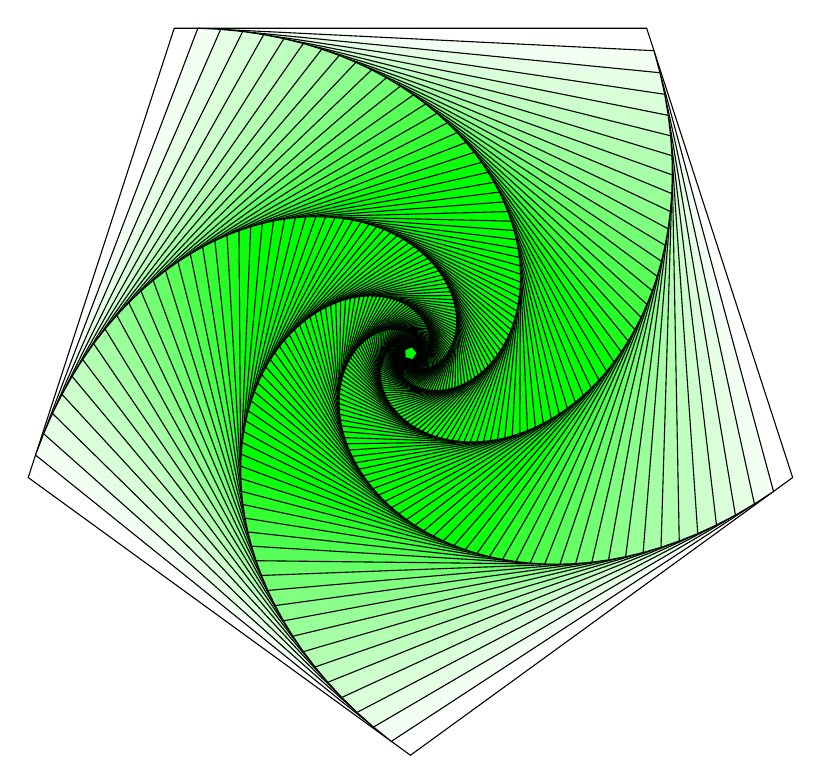
\begin{tikzpicture}
    \def\couleur{green}
    \path[coordinate] (0,0)  coordinate(A)
                ++( 144:6cm) coordinate(B)
                ++(72:6cm) coordinate(C)
                ++(0:6cm) coordinate(D)
                ++(-72:6cm) coordinate(E)
                                ;
    \draw[fill=\couleur!\thedensity] (A) -- (B) -- (C) --(D) -- (E) --  cycle;
    \foreach \x in {1,...,120}{%
        \pgfmathsetcounter{density}{\thedensity+5}
        \setcounter{density}{\thedensity}
        \path[coordinate] coordinate(X) at (A){};
        \path[coordinate] (A) -- (B) coordinate[pos=.05](A)
                            -- (C) coordinate[pos=.05](B)
                            -- (D) coordinate[pos=.05](C)
                            -- (E) coordinate[pos=.05](D)
                             -- (X) coordinate[pos=.05](E);
        \draw[fill=\couleur!\thedensity] (A)--(B)--(C)-- (D) --(E)  -- cycle;
    }
\end{tikzpicture}

\end{centering}
\begin{centering}

\tikzstyle{level 1}=[sibling angle=120]
\tikzstyle{level 2}=[sibling angle=60]
\tikzstyle{level 3}=[sibling angle=30]
\tikzstyle{every node}=[fill]
\tikzstyle{edge from parent}=[snake=expanding waves,segment length=1mm,
                              segment angle=10,draw]
\begin{tikzpicture}[grow cyclic,shape=circle,very thick,level distance=13mm,
                    cap=round]
\node {} child [color=\A] foreach \A in {red,green,blue}
    { node {} child [color=\A!50!\B] foreach \B in {red,green,blue}
        { node {} child [color=\A!50!\B!50!\C] foreach \C in {black,gray,white}
            { node {} }
        }
    };
\end{tikzpicture}
\end{centering}

\newpage

\begin{centering}
\begin{Large}
\textbf{《圣经:创世纪》节选}
\end{Large}\vsp
\large

起初,神创造逻辑。

逻辑是空虚的。

神的零运行在水面上,

这是平凡的。

神说,要有集合。

于是就有了集合。

神看集合是好的,

就将其公理化。

有集合,有运算,

就是一个代数结构。\vsp

神照自己的样子造人,

于是就有了0.

神在东方的伊甸建立了一个园子,

称之为群。

神将0安置在那里,

让它作幺元。

起初,伊甸园是平凡的。

神说,园中所有果子你可以随便吃。

只有后继树上果子,你不能吃。

因为你吃的时候必死。\vsp

神说,那人独居不好。

于是要为它造一个配偶。

神让0沉睡,取它的后继数1.

神把1带到伊甸园,

让它和0配对,

二人从此一起生活。

神教给它们加法的运算,

让它们可以互相交合。

0依然是伊甸园的单位元。

0的逆元是0,1的逆元是1,

0和1彼此交合则又得到1.\vsp

神所造的,

惟有皮亚诺比一切的活物更狡猾。

皮亚诺对1说,

神岂是真说不许你们吃园中所有树上的果子么?

1对皮亚诺说,

园中树上的果子我们可以吃,

唯有后继树上的果子不可,

免得我们死。

皮亚诺说,你们不会死。

神是怕你们吃了后继树上的果子,

能自己创造新的数。\vsp

皮亚诺告诉1它自己是怎么来的,

1对单调的只有0和1的加法已经厌烦。

它看后继树上的果子可做食物,

而且悦人眼目,是可喜爱的,

就摘下果子来吃了。\vsp

于是1对自己取了后继数,是为2.

1又摘下果子给2,2也吃了。

于是2对自己取了后继数,是为3.

很快,后继树下生成了所有正整数。。。

\end{centering}
\vspp

\begin{center}
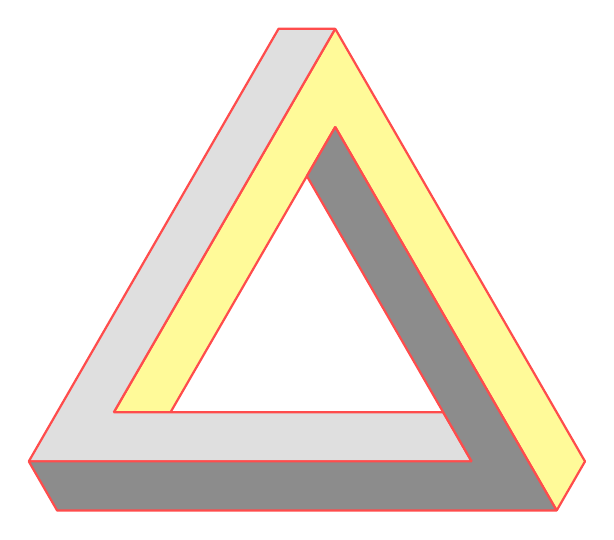
\begin{tikzpicture}[scale=0.8, line join=bevel]
    \pgfmathsetmacro{\a}{2.5}
    \pgfmathsetmacro{\b}{0.9}

    \tikzset{%
      apply style/.code     = {\tikzset{#1}},
      triangle_edges/.style = {thick,draw=red!70}
    }
    \foreach \theta/\facestyle in {%
        0/{triangle_edges, fill = yellow!40},
      120/{triangle_edges, fill = gray!25},
      240/{triangle_edges, fill = gray!90}%
    }{
      \begin{scope}[rotate=\theta]
        \draw[apply style/.expand once=\facestyle]
          ({-sqrt(3)/2*\a},{-0.5*\a})                     --
          ++(-\b,0)                                       --
            ({0.5*\b},{\a+3*sqrt(3)/2*\b})                -- % higher point	
            ({sqrt(3)/2*\a+2.5*\b},{-.5*\a-sqrt(3)/2*\b}) -- % rightmost point
          ++({-.5*\b},-{sqrt(3)/2*\b})                    -- % lower point
            ({0.5*\b},{\a+sqrt(3)/2*\b})                  --
          cycle;
        \end{scope}
      }	
\end{tikzpicture}
\end{center}






